% A simple LaTeX template for lab reports....
\documentclass[abstract=on]{scrreprt}
%\documentclass{amsart}
\usepackage[utf8]{inputenc}
\usepackage[margin=1.25in]{geometry} %page margins
\usepackage{lipsum}
\usepackage[usestackEOL]{stackengine}
\setcounter{secnumdepth}{5} %include numbering of subsubsubsusbsusbsections!
\setcounter{tocdepth}{5}% Include \subsubsubsusbsusbsection in ToC!


\usepackage{wrapfig} %wrap text around pics

%linked TOC
\usepackage{hyperref}
\hypersetup
{
    colorlinks,
    citecolor=black,
    filecolor=black,
    linkcolor=black,
    urlcolor=black
}

\usepackage{natbib}
\usepackage{graphicx}
%\usepackage{titlesec}
\usepackage{url}
%\usepackage[backend=bibtex]{biblatex}
%\usepackage[acronym]{glossaries} %only interested in loading acronym-part
\usepackage[printonlyused,withpage]{acronym}

%\usepackage[printonlyused]{acronym}

%------ Listings --------------
\usepackage{color}
\definecolor{light-gray}{gray}{0.95}
\definecolor{orange}{rgb}{1, 0.5, 0}

\definecolor{gray75}{gray}{0.75}
\definecolor{gray1}{gray}{0.97}
\definecolor{gray2}{gray}{0.90}
\definecolor{gray3}{gray}{0.80}
\definecolor{gray4}{gray}{0.63}

\usepackage{caption}
\DeclareCaptionFont{white}{\color{white}}
\DeclareCaptionFormat{listing}{\colorbox[cmyk]{0.0, 1.0, 0.7,1.0}{\parbox{\textwidth}{\hspace{15pt}#1#2#3}}}
%\captionsetup[lstlisting]{format=listing,labelfont=white,textfont=white, singlelinecheck=false, margin=0pt, font={bf,footnotesize}}



\usepackage{natbib}

% Edit the meta.tex file to change title, group number and author names
% Fill in the report title, group number and student names here
\newcommand{\mytitle}{Something about an LNA for neural interfaces and shit in the face}
%\newcommand{\mygroupnumber}{1}
\newcommand{\myauthor}{Bengt Erik Hope}

\title{\mytitle}
\author{\myauthor}
\date{\today}



\pagenumbering{gobble} %%disable pagenumbering
\begin{document}
% The title page, edit if you want to customize it
\begin{titlepage}

\includegraphics[height=1.5cm]{images/ntnu_logo.pdf}\\[1cm]   
\begin{center}

 
% Upper part of the page
~\\[1.5cm]

\textsc{\Large - TFE4520 - \\Project Report}\\[0.5cm]

% Set the title of the Document between two horizontal lines
\hrule ~\\[0.2cm]
{\huge \bfseries \mytitle}\\[0.4cm]		% print the title of the document
\hrule ~\\[1.5cm]

% Additional Information about the document
\begin{minipage}{0.4\textwidth}
    \centering
	\large
%		\emph{Group \mygroupnumber:}\\~\\
		\myauthor
\end{minipage}

\vfill

% Bottom of the page
{\large \today}

\end{center}
\end{titlepage}

% Main matter - edit corresponding file under content/ to change
\begin{abstract}
%An abstract is a short (100 to 500 words), high-level summary of the entire document. 
%For this kind of report, you would start by introducing the concept that the report talks about and the goals of the work, followed by information about how the work was done and some summary of results.
TheDesignofIntegrated
CircuitstoObserve
BrainActivity

%\smallskip
%\noindent \textbf{Keywords.} list of keywords

%{\bf Keywords:} keyword A, keyword B
\lipsum[1-2]
{\raggedleft\vfill\itshape\Longstack[l]{%
  I've always wanted an
  apple corer.\\ \\
  - Shithead
}\par
}
%\small\hfill KeykeywordA, keywordB ,keywordC
\end{abstract}


%%init TOC
\newpage
  \tableofcontents
 % \setcounter{tocdepth}{5}
  
\newpage
  %%Acronyms
  \section*{List of Acronyms}
  \begin{acronym}
    \acro{LNA}{low noise amplifier}
    \acro{ECoG}{electrocorticography}
    \acro{EEG}{electroencephalography}
    \acro{iEEG}{intercranial electroencephalography}
    \acro{IC}{integrated circuit}
    \acro{CMOS}{complementary metal-oxide-semiconductor}
    \acro{LFP}{local field potentials}
    \acro{MEMS}{microelectromechanical system}
    \acro{ADC}{analog to digital converter}
    \acro{CMRR}{common mode rejection ration}
    \acro{BMI}{brain-machine interface}
  \end{acronym}

\newpage

%\thispagestyle{empty}
\listoffigures
\newpage

%\listoftables
%\newpage
\pagenumbering{arabic} %%enable page numbering

\chapter{Introduction}
The main objective for this report is to propose a \acf{LNA} front-end for extracellular\footnote{\emph{extracellular} means "outside the cell"} in-vito\footnote{\emph{in-vivo} is Latin for "within the living"}
neural signal recording electrodes, as well as to research what requirements can be considered critical in achieving such a design. As a natural consequence of the main objective, the project - which this report is a
product of - will explore the usage of \acs{CMOS} technology in neural recording systems. Any findings produced can therefore be used as a preliminary for further research in the authors upcoming graduate thesis. 
Thus, some basic elaborations on where the design can potentially be situated in a complete \acf{BMI} - such as a bio-medical \acs{IC} or a neuro \acs{MEMS} array with fully integrated electronics, will be undergone. \\*

The rest of this chapter will describe the motivation for initiating this project, provide a rudimentary overview of past work in this area, mention outcomes of the project, and outline the structure of the rest of the report.

\section{Motivational Background}
Technological advances towards a type of electromechanical or biomedical augmentation of the human body which remedies,
    improves or maybe even grants the user a new set of abilities are intriguing thoughts for anyone with a little \emph{cyberpunk} in them. There is still
    quite a long way before any such leaps in technology are possible. However, forcing oneself into more pragmatical ways of thinking; there is no doubt that demands for technologies enabling scientists and clinicians to record neural activity from a large number of neurons in a brain is continuously rising. Namely collecting high temporal and spatial resolution neural data from micromachined multielectrode arrays is something that can be regarded standard practice in basic neuroscientifical research \cite{harrison2003low}. Such research is starting to enable medical, as well as neuroprosthetic applications, and we see that neural recordings can provide scientific insight into the neural correlates of cognitive, sensory and motor processes \cite{miller2007spectral,chang2010categorical,gunduz2011neural}. Experiments and clinical trials with primates - both human \cite{hochberg2006neuronal} and non-human \cite{wessberg2000real}, as subjects have shown that data directly derived from signals - namely action and \acl{LFP}s (which are to be discussed in chapter \ref{chap:two}), can be used to control robotic prosthetics.

    In the efforts to implement wholly implantable devices for neural recording purposes, \acf{MEMS} electrode arrays can be complimented with \acf{CMOS} \acl{IC}s in such a way that one achieves parallel stand-alone \acs{BMI}s with on-board wireless data and power transfer, as well as \acs{ADC}s and a processor \cite{najafi1986implantable,wise2004wireless,olsson2005three}. The continuously improving resolutions of \acs{MEMS} arrays have enabled simultaneous recording of large neuron populations with spatial resolutions down to a single cell activity from populations of neurons \cite{kipke2003silicon}.

    Studies such as the ones mentioned have shown a promising future for developing \acs{BMI}s that have practical use for humans. But to reach that point in the future where such systems can be implanted in-vito in humans and function symbiotically with them in their everyday activities, many challenges must be overcome. 
%--------------------------figure-------------------------------------------------------------------
    \begin{figure}
	\centering
	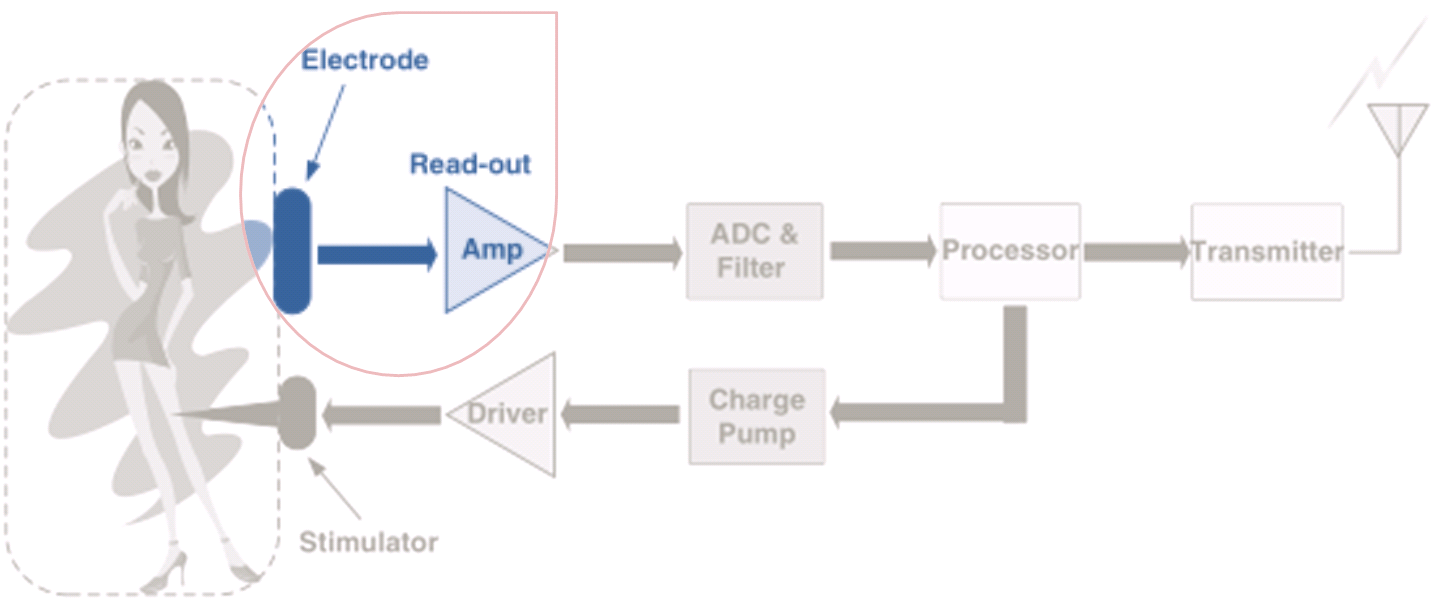
\includegraphics[scale=.4]{images/block-bio-medical-subsystem.png}
	\caption{\texttt{\footnotesize{typical architecture of bio-medical \acs{IC} subsystem \cite{yoo2011biomedical-cmos}}}}
	\label{fig:block-arch-biomedical-subsystem}
    \end{figure}       
%--------------------------END-------------------------------------------------------------------
%--------------------------figure-------------------------------------------------------------------  
\begin{wrapfigure}{r}{5.7cm}
  \vspace{-20pt}
  \caption{\texttt{\footnotesize{block diagram of a wireless neural recording device}}}
  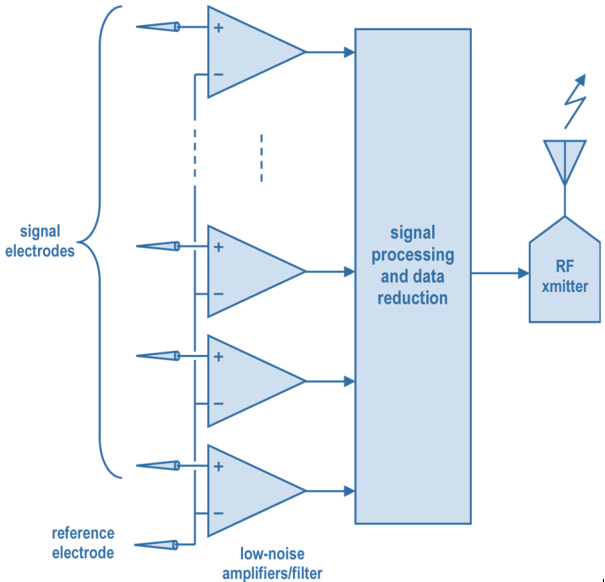
\includegraphics[width=5.7cm]{images/block-wirelss-neural-rec-dev.png}
  \vspace{-30pt} 
  \label{fig:block-neural-recording-dev}
\end{wrapfigure} 
%--------------------------END------------------------------------------------------------------- 
    Even though we are limited to propose a preliminary design for a \acl{LNA} front-end for neuro-probes with a type of platinum/iridium based electrodes, we will explore requirements to make the design compatible for integration in a complete in-vito \acl{BMI} which utilizes a \acs{MEMS} electrode array based transducer. The research in this area will ideally continue in the authors upcoming graduate thesis. A block diagram illustrating our focal point in a complete biomedical \acs{IC} - which also has an interface for stimulation, is shown in figure \ref{fig:block-arch-biomedical-subsystem}. Also, a block diagram depicting the principle for a multielectrode wireless neural interface is given in figure \ref{fig:block-neural-recording-dev}.
  
\section{Past Work}
    %refer MIT thesis
There is much literature describing both conceptual and physical implementations neural recording systems with varying degrees of practical usability. derpa derp...%TODO:

\section{Summary of Authors Contributions}
  \begin{itemize} 
    \item nada
    \item nuthin'
  \end{itemize}

\section{Report Outline}
The report is organized in the following manner:
  \begin{itemize}
    \item \textbf{Chapter 2} briefly presents the motivational background for neural recording before digging into the relevant theory needed to understand the design 
		  itself as well as eventual limitations and difficulties in realizing the best possible specifications. 
		  It also provides a basic theoretical understanding of the neural recording principles from an electronic designers point of view - namely how \acs{LNA} to interface
		  with intercranial electrodes.
    \item \textbf{Chapter 3} TODO
    \item \textbf{Chapter 4} TODO
  \end{itemize}
 
\chapter{Theoretical Background \& Literature Review}
\label{chap:two}
 
 As mentioned, this reports main focal point will be on the design of a \acs{LNA} front-end for a transducer utilizing a type of platinum-iridium based electrodes. 
 As such we will start exploring basic characteristics of neural signals and some practicalities on recording them, before we dig into the electronics theory necessary for us to determine a design methodology for the neural interface front-end. Notice also that remarks about the amplifier design - which is to be fully introduced in later chapters, are made as the theory discussion progresses.
 
  \section{Neural Recording through Biopotential Acquisition}
  \label{sec:biopotential-aquisition}
  Neural recording devices basically performs biopotential acquisition using transducers that converts ionic conduction to electronic conduction so that biopotential 
  signals can be stored and viewed. The biopotential signals themselves are generated due to electrochemical activity of electrogenic cells\footnote{\emph{Electrogenic cells} 
  refers to cells that exhibit the ability to generate electrical signals\cite{GBM8320-2013-electrodes-ch8-pt1}} - such as neurons, that are components of muscular, 
  nervous or glandular tissue. There are several measurement variations that are relevant for collecting biopotential data, whereas the ones considered most relevant 
  for the scope of this report are \emph{\acf{EEG}}, \emph{\acf{ECoG}} and \emph{\acf{iEEG}} (also commonly referred to by the somewhat misleading term \emph{\acf{LFP}}).
  
    From a historical perspective one usually refers to surface recording - that is, placing electrodes on top of the scalp - as \acs{EEG}, while \acs{ECoG} and \acs{iEEG} have coined the use of in-vivo
  intercranial electrodes in order to record electrical activity in the brains cerebral cortex\footnote{The \emph{cerebral cortex} is the outermost sheet of neural tissue covering the cerebral hemispheres in mammals. \cite{marcus2014future}}.
	More specifically on in-vivo recording; \acs{iEEG}\textbackslash\acs{LFP} is usually referred to when recordings are performed using small electrodes placed directly into the cortex from beneath the skull,
  while with \acs{ECoG} recordings one places the electrodes on the surface of the cortex.%\\*  
  
  
    \subsection{The Neural Signals}
     \label{subsec:neural-signals}
    We have have explained that there exists multiple measurement types for recording cortical activity. Biopotential signals generated by electrogenic cells like neurons, produce voltage changes on the order of 100 mV relative to the extracellular fluid \cite{kandel2000principles}. Collecting measurements of this type is possible in brief periods of time by carefully directing individual placement of microelectrodes intracellularly\footnote{\emph{Intracellular} means "inside the cell"}. To get around the limitations of only detecting single cells at a time - and for such short durations, the prime methodology at present is using microelectrode arrays extracellularly (though there exists rudimentary initiatives to merge the advantages of extracellular microelectrode arrays and intracellular microelectrodes, they have still not gained significant usability) \cite{spira2013multi}. A trade-off here is that we accept "blindness" to potentials generated by single cells as well as a significant reduction in signal amplitude. However, an interesting relationship is shown in figure %--------------------------figure-------------------------------------------------------------------        
    \begin{wrapfigure}{r}{4.5cm}
      \vspace{-20pt}
      \caption{\texttt{\footnotesize{Rec. of action potential}}}
      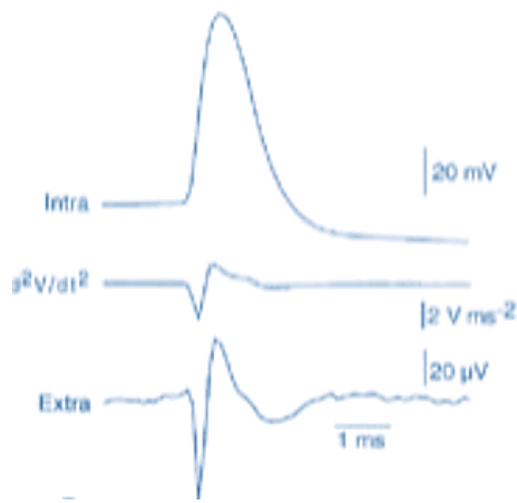
\includegraphics[width=4.5cm]{images/intracellular-amp-vs-extracellular-amp.png}
      \vspace{-25pt} 
      \label{fig:intracell-vs-extracell}
    \end{wrapfigure}
%--------------------------END-------------------------------------------------------------------
\ref{fig:intracell-vs-extracell} (adapted from \cite{extracell-action-pot-2009}); we can see that the shape of the extracellular voltage potential qualitatively matches the second time derivative of the intracellular voltage potential \cite{cohen2000contributions}. Note that the resulting variation in cellular potential with time is known as the action potential \cite{GBM8320-2013-electrodes-ch8-pt1}. Action potentials can be interpreted as "digital" events  - neurons normally induce spikes of similar amplitudes and time durations, and information is said to be found in the timing of these "digital" events \cite{harrison2008design}.
    
    A measurement type can be characterized by their signal strength (which we can see from fig.\ref{fig:cortical-measurements} is usually in the $\mu$-volts range) and surgical invasiveness 
    versus frequency and electrode area. This is presented in figure \ref{fig:cortical-measurements}.   
%--------------------------figure-------------------------------------------------------------------        
      \begin{figure}
	\centering
	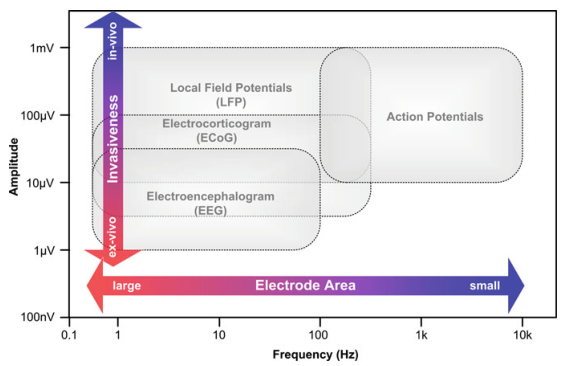
\includegraphics[scale=.75]{images/Amp-vs-freq-common-biopotential-signals2.png}
	\caption{\texttt{\footnotesize{different cortical measurements \cite{yoo2011biomedical-cmos}}}}
	\label{fig:cortical-measurements}
      \end{figure}
%--------------------------END-------------------------------------------------------------------
    \acs{ECoG} signals is measured using subdural surface electrodes (refer to 1. on fig.\ref{fig:neural-probe}). This type of measurement is outside of our design scope due to frequency range,
    but it can be mentioned that the method offers significant increase in spatial and temporal resolutions as well as stronger amplitudes - especially in 
    the high gamma frequency range\footnote{Gamma frequency ranges between ~70Hz to ~110Hz\cite{hill2012recording}}, 
    in contrast to the non-invasive surface based \acs{EEG} topologies \cite{hill2012recording}. This leads us to the very similar \acs{LFP} signals.
    \acs{LFP} oscillations differs from \acs{ECoG} in that LFPs are recorded from within the cortical tissue (illustrated by 2. in fig.\ref{fig:neural-probe}). 
    It is considered the internal correlate of \acs{ECoG} as it registers as the same "crowd noise" - that is synchronous activity of many neurons in one region of the brain,
    as ECoG recording, only with substantial blurring and attenuations. The signal deterioration happens because LFP oscillations is usually measured using microelectrode arrays \cite{harrison2008design}. This means LFP spectra is unavoidably detected with microelectrode arrays, even though one might only be after action potentials. It is, however, often beneficial to record both LFP together with action potential spikes and then apply linear filtering - which should be fairly easy to achieve considering frequency ranges are mostly different for the two signal types. LFPs are interesting for the same reasons that ECoG signals are; they have among other things been especially suitable in understanding motor movements of the body \cite{donoghue1998neural} and are consequently very suitable for e.g. neuroprosthetic applications.
    
    We notice from figure \ref{fig:cortical-measurements} that the low frequency characteristics and small signal amplitudes poses strict 
    noise requirements on designing a \acl{LNA}. In addition we know that \acs{CMOS} low noise design at such low frequencies will not
    be a straightforward experience because of \acs{CMOS} circuitry's susceptibility to flicker noise. For the \acs{LNA} design - which is to be introduced
    next chapter, we will focus on action potential measurements. Therefore flicker noise should be a little less of a problem for us as we are in the 100 Hz to 10 kHz 
    frequency range. We will however, have to deal with a larger impedance because smaller electrode area is needed to measure action potentials.
    Also an important remark to make is about eventual LFP signals; as it is assumed that our LNA will be used for interfacing with a microelectrode array, LFP parts ($<$ $\approx$200 Hz) in the recording
    would be amplified and they would have be filtered out at a later stage in the system if they are unwanted.
    
    Fig.\ref{fig:cortical-measurements} also tells us something of what \acf{CMRR} we have to expect from the LNA. Again we focus on action potentials and see that the frequency of interest is higher than e.g. the mains frequency for instance, so we can have a much more relaxed \acs{CMRR} than any other type of neural recording. We still need to try to minimize capacitive and inductive interferences though. In addition; tethering forces introduced by conductors will cause problems for electrodes inserted into the sensitive tissue of the brain. Therefore one should ideally place the amplifier as close to - ideally directly attached to, the transducer. A guideline summary of LNA design considerations in regards to what type of neural signal one seek to record is given in \cite{yoo2011biomedical-cmos} and illustrated in figure \ref{tab:lna-design-considerations}.
%--------------------------figure-------------------------------------------------------------------      
    \begin{figure}
      \centering
      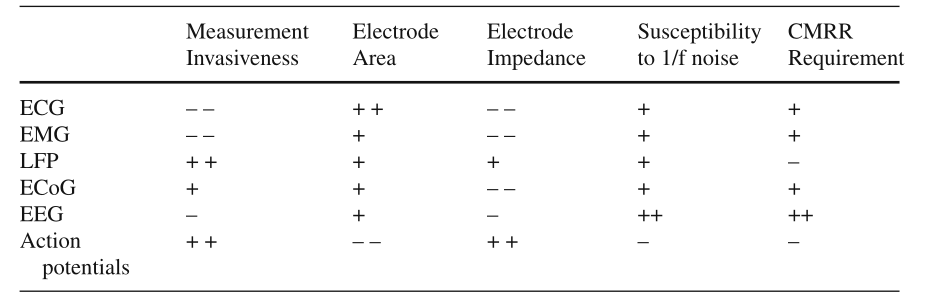
\includegraphics[scale=.5]{images/table-LNA-design-considerations.png}
      \captionsetup{singlelinecheck=off}
      \caption[dummy]{\texttt{\footnotesize{Summary of the considerations during the design of instrumentation amplifiers for different neural signals.\\
					      (-) indicates a low/small value \\
					      (+) indicates a high/large value}}}
      \label{tab:lna-design-considerations}
      \end{figure}
%--------------------------END-------------------------------------------------------------------              
       
    \subsection{Real-life Application of ideal Polarizable \& Non-Polarizable Electrodes} %%refer 4.2 in bimedical cmos
    \label{subsec:electrodes}
    To be able pick up biopotential-signals, current should flow from the tissue into the acquisition electronics. As the current is carried by ions in the body of a living being, a transducer is needed to convert ionic current into electronic current.\\*\\*
    Enter the \textbf{electrode}.\\ %See figure \ref{fig:neural-probe}\\
%--------------------------figure-------------------------------------------------------------------
    \begin{wrapfigure}{r}{0.5\textwidth}
      \centering
      \vspace{-20pt}
      \caption{\texttt{\footnotesize{electrode model}}}
      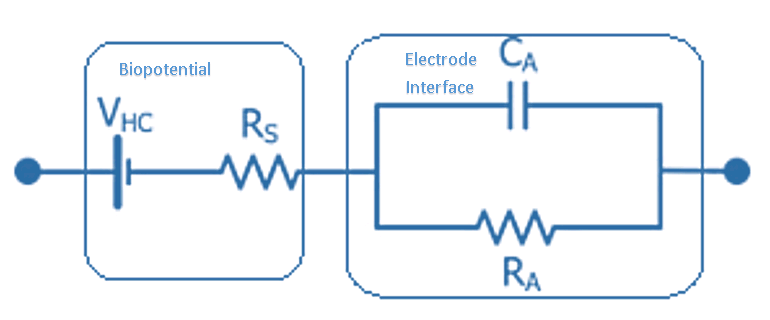
\includegraphics[width=0.5\textwidth]{images/electrical-probe-model1.png}
      \vspace{-35pt}
      \label{fig:probe-model}h
    \end{wrapfigure}
    \begin{wrapfigure}{r}{0.5\textwidth}
      \centering
      \vspace{-20pt}
      \caption{\texttt{\footnotesize{electrode array model}}}
      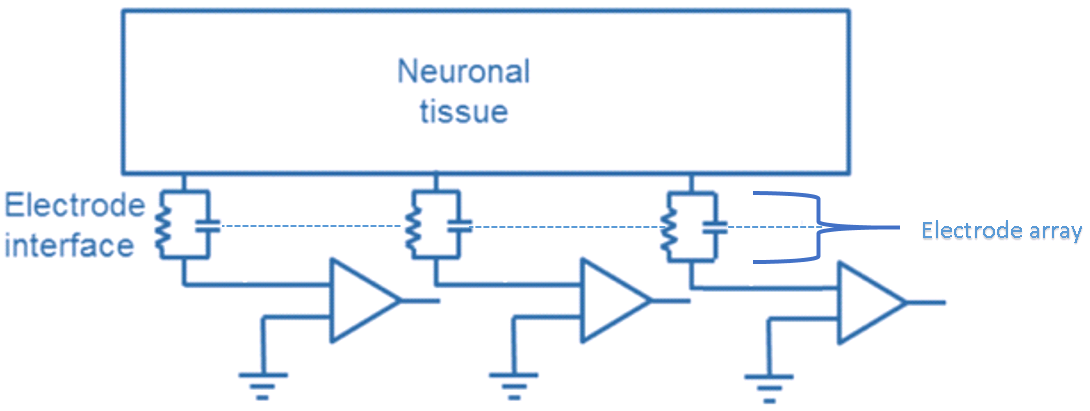
\includegraphics[width=0.5\textwidth]{images/electrical-probe-model-arrays.png}
      \vspace{-20pt}
      \label{fig:probe-model-array}
    \end{wrapfigure}
%--------------------------END-------------------------------------------------------------------  
    How easily electrons travel through the electrode interface defines if the electrode is considered non-polarizable or polarizable. If current flow 
    happens by very little energy, the electrode is referred to as being non-polarizable.  As such the electrode would ideally see no over-potentials and 
    thus, a \emph{perfectly} non-polarizable electrode can be seen as a simple resistor. If no charge crosses the electrode transfer, the electrode is 
    referred to as polarizable and can ideally be seen as capacitor as we only have a displacement current.
%--------------------------figure-------------------------------------------------------------------      
    \begin{figure}
      \centering
      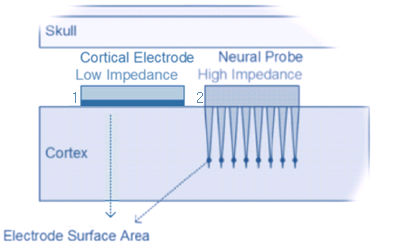
\includegraphics[scale=.7]{images/probe-placement2.png}
      \captionsetup{singlelinecheck=off}
      \caption[dummy]{\texttt{\footnotesize{       				    
						    \begin{enumerate}
						      \item Cortical or subdural electrode placed under the skull directly on the surface of the brain.
						      \item Neuro-probe array placed on the surface of a brain. The recording electrodes are drawn as dots on the array of probes penetrating the cortex
						    \end{enumerate}}}}
      \label{fig:neural-probe}
      \end{figure}
%--------------------------END------------------------------------------------------------------- 
    However, the real world is not so forgiving; no electrode is purely polarizable or non-polarizable, rather something in between. We therefore present a 
    basic electrical model of a single electrode \cite{GBM8320-2013-electrodes-ch8-pt1} shown in figure \ref{fig:probe-model}.
    We see from \ref{fig:probe-model} that the source impedance can be modeled by a Thevenin equivalent source with a source impedance of Rs, while the electrode can be 
    modeled by a capacitor C\textsubscript{A} in parallel with a resistor R\textsubscript{A}.   
 
    Notice from figure \ref{fig:neural-probe} how the different electrode placement generally cover different areas. The impedance of an electrode plays an 
    important role during the design of the recording circuit when selecting amplifier design topology. We know that as the electrode surface 
    area decreases, its impedance tends to increase \cite{yoo2011biomedical-cmos}. Thus, the use of probes with high small electrode area
    forces us to design an amplifier with high input impedance.
   
   
   \section{Transistor and Amplifier basics}
    \label{subsec:trans-amp-basics}
      \subsection{Noise Performance}
	\subsubsection{Noise Figure}
%    	\[f_{DAC} = f_{HFPERCLK}  \frac{1}{2^{PRESC}}\]
        
%        bla bla bla derp dahsd
%        \begin{gather}
%        \label{cycle-formula}
%            \Delta C = \frac{f_{HFCORECLOCK}}{f_{samplerate}} = \frac{14000000}{44100} \approx 317
%        \end{gather}
%        tralalalla halo aodhnag
        
	\subsubsection{Noise Efficiency Factor}
	%TODO:
	In order to be able to compare the noise specifications
reached with other recently published IAs, a noise efficiency factor (NEF) is introduced. The total equivalent
input noise of an ideal bipolar transistor (only thermal
noise and no base resistance) is given by

2015HoST Project noise noiseEffFactor

with BW being the frequency bandwidth (for a bipoku
transistor this is the ft). The NEF of a system is then
defined as

2015HoST Project noise noiseEffFactor

where In, is the total current drain in the system and

Vi. is the total equivalent input noise. The NEF describes how many times the noise of a system with the
same current drain and bandwidth is higher compared to
the ideal case, e.g., for a CMOS transistor with only white
noise, the noise power is given by

2015HoST Project noise noiseEffFactor

  
\chapter{The LNA front-end}
Given that the \acl{LNA} makes up the first stage in a neural recording device, it easily becomes one of the most important modules in it.  We discovered in chapter \ref{chap:two} that when interfacing with a \acs{MEMS} array - which has become our transducer of interest, we have the ability to amplify both action potentials and \acs{LFP}. We discussed that our design scope will be limited for action potentials and therefore have a more relaxed CMRR than we would have if we were interested in the LFPs. This led us to remark that the amplifier preferably should be attached to the transducer itself. Such a placement compels us to consider another requirement - namely heat dissipation. Findings in  \cite{seese1998characterization} tells us that cells exposed to certain temperatures over prolonged periods of time simply dies. Thus, we will have to limit amplifier power usage.  \cite{harrison2008design} claims that modern \acs{MEMS} arrays consists of something like 100 electrodes and that a 6 x 6 x 2 $mm^3$ must then consume less than 100$\mu$W. We can summarize design requirements as follows:

\begin{enumerate}
  \item\textbf{Dynamic range} - Fig.\ref{fig:cortical-measurements} indicates that we must have a dynamic range good enough to convey action potentials as low as \mp2mV.
  \item\textbf{Input Impedance} - Higher input impedance than the transducer as well as negligible dc input current.
  \item\textbf{Bandwidth} - 100-10kHz to pick up action potentials.
  \item\textbf{DC offset} - block DC offset at the transducer to prevent unwanted saturation of the amplifier.
  \item\textbf{Noise} - input noise must be small enough to pick up amplitudes as small as $\simeq$30$\mu$V
\end{enumerate}

\chapter{Design Methodology}
This chapter should discuss the details of your implementation for the assignment.
Everything related to \emph{how} things were done should go here.
Remember to avoid going into too much details, summarize appropriately and try to use figures/charts.
Make sure you refer to the figures (such as Figure %\ref{fig:universe}) and charts you add in the text.
Avoid putting lots of source code here -- small code snippets are fine if you want to discuss something specific.


\section{Amplifier Topology}
Add content in this section that describes how you tested and verified the correctness of your implementation, with respect to the requirements of the assignment.
\chapter{Results}
In this chapter, you should discuss the results you have obtained from your implementation.
These can be correctness results, i.e whether the implementation behaved as expected, or numerical results that express runtime or energy measurements.
\chapter{Conclusion}
This chapter should be a look back at the entire report and summarizing the problem, the solution and the obtained results.

\section{Evaluation of the Assignment}
You can include comments about the assignment itself here. While this part is not obligatory and not graded, it is valuable feedback to the course staff that can be used to improve the exercises in the future.

% Bibliography - edit references.bib and use the \cite command in text
\bibliographystyle{plain}
\bibliography{references}
\end{document}
